% !TEX root = ./thesis.tex
%\documentclass[phd]{pacotes/unb-cic}
\documentclass[bacharelado]{packages/unb-cic}%

%\usepackage[none]{hyphenat} %% diable hyphen
% \usepackage{fontspec} % MacOS
\usepackage[table]{xcolor}% http://ctan.org/pkg/xcolor
\usepackage[american,brazil]{babel}
\usepackage[T1]{fontenc}
\usepackage{indentfirst}
\usepackage{natbib}
\usepackage{xcolor,graphicx,url}
\usepackage[utf8]{inputenc}
\usepackage{booktabs} % for tables
\usepackage{verbatim} %% multiline comments
\usepackage{dirtytalk} %% Quotes

\usepackage{epsfig}

\usepackage{listings}
\usepackage{packages/tikz-uml}

%% Algorithm
\usepackage[ruled,linesnumbered]{algorithm2e}
\usepackage{float}
\newfloat{algorithm}{t}{lop}
\floatname{algorithm}{Algorithm}
%% End Algorithm

%% definitions
\usepackage{amsmath}
\newtheorem{thm}{Theorem} % reset theorem numbering for each chapter
\newtheorem{defn}[thm]{Definition} % definition numbers are dependent on theorem numbers
%% end definitions

\graphicspath{ {imagens/} } % path to images

%\bibpunct[; ]{(}{)}{,}{a}{}{;}%muda colchetes para parenteses

% definicoes previas do documento
%\selectlanguage{brazil}
\title{GoalD: Autonomic Goal-Driven Deployment in Heterogeneous Computing Environments}

\orientador[a]{\prof[a] \dr[a] Genaina Nunes Rodrigues}{CIC/UnB}

\coordenador[a]{\prof[a] \dr[a] Célia Ghedini Ralha}{CIC/UnB}

\diamesano{16}{Dezembro}{2020}


\membrobanca{\prof[a] \dr[a]  Célia Ghedini Ralha}{CIC/UnB}
\membrobanca{\prof \dr Raian Ali}{Bournemouth University}

\autor{Gabriel Siqueira}{Rodrigues}

\CDU{004.4}

\palavraschave{dependabilidade}
\keywords{dynamic deployment, heterogeneous computing environment, context- and goal-oriented requirements engineering}

%-------------------------------------------------

\begin{document}

\maketitle

\pretextual
%\begin{agradecimentos}
%Agradecemos à nossa orientadora, \prof[a] \dr[a] Genaina Nunes Rodrigues,
%\end{agradecimentos}

%\begin{resumo}
%Nesse trabalho apresentamos...
%\end{resumo}

\selectlanguage{american}

\begin{abstract}%\textbf{}

% \input{parts/abstract}

\end{abstract}

%\selectlanguage{brazil}
\tableofcontents
\listoffigures
%listoftables

\textual

\chapter{Introduction}
\label{chap:introduction}
Sistemas Multi-Robôs (SMR) são sistemas que consistem em mais de um agente robótico. Por algumas décadas esses sistemas foram utilizados em diversos contextos para cumprir diversas tarefas, especialmente em ambientes dinâmicos. SMRs atuam em um espaço ciber físico (i.e. parte do “mundo real”), logo seus agentes estão propensos à mudanças provenientes tanto de outros agentes do sistema como do ambiente em que estão inseridos \cite{iocchi2000reactivity}. Para aumentar a adaptabilidade do SMR, pode-se projetá-lo como um sistema auto-adaptativo, tornando-o capaz de responder à mudanças no ambiente, de maneira a continuar cumprindo objetivos e respeitando os limites impostos ao sistema \cite{sykes2010autonomous}.

Os agentes desses sistemas (i.e. robôs) existem no mundo físico e interagem com ele e entre si de maneiras mais complexas do que agentes de outros sistemas (e.g. computadores, bancos de dados, etc) \cite{cao1997cooperative}. Isso traz desafios para o desenvolvimento desse tipo de sistema, principalmente a preparação de experimentos com vários robôs \cite{noori20173d}. Essa dificuldade pode ser superada com o uso de simuladores.

Simuladores podem ser empregados tanto para testar a segurança, eficiência e robustez do sistema, quanto para prototipação de SMRs e robôs \cite{noori20173d}, \cite{pinciroli2012argos}. Outras vantagens de simuladores incluem: 

\begin{itemize}
    \item Menor custo de tempo e recursos para preparação e execução do experimento
    \item Ambientes simulados podem ser mais ricos, complexos e seguros que ambientes reais ou em laboratório \cite{robotSimulation}
    \item é possível testar hardware que não está disponível \cite{pinciroli2012argos},  \cite{echeverria2011morse}, \cite{robotSimulation}
\end{itemize}

De acordo com o Survey realizado \cite{robotSimulation}, muitos desenvolvedores de sistemas robóticos confirmam que simulações são ferramentas populares entre eles e um dos casos de uso mais comuns são os testes.

Diversos simuladores para SMRs existem na literatura, por exemplo Gazebo \cite{koenig2004gazebo}, Simbad \cite{hugues2006simbad}, CoppeliaSim \cite{rohmer2013coopeliasim}, MORSE \cite{echeverria2011morse} e Dragonfly \cite{maia2019dragonfly}, entre outros. Cada um desses simuladores foi criado com propostas diferentes, desde simulação precisa das partes que compõem um robô e sua interação com o ambiente (Gazebo, CoppeliaSim, Morse), até simulações de mais alto nível focando principalmente no comportamento dos robôs (Simbad, Dragonfly). Simulações multi-robô são suportadas por simuladores atuais, mas geralmente em menor número - devido ao alto uso de recursos computacionais necessários para simular cada robô (i. e. experimentos feitos com Gazebo mostraram que o simulador tem dificuldades ao simular mais de 10 robôs \cite{noori20173d}) - ou são muito específicos quando conseguem simular mais robôs (i.e. Dragonfly supostamente é capaz de simular até 400 entidades, mas está restrito à simulação de drones \cite{maia2019dragonfly}).

Ainda que simulações tenham um bom potencial, testes de campo são mais utilizados para validação e para verificação em sistemas robóticos do que os testes baseados em simulações. Alguns problemas dificultam o uso de simulações para fazer a validação e verificação (V\&V), dentre eles \cite{robotSimulation}:
\begin{itemize}
    \item Não ser possível ou dar muito trabalho para testar a aplicação com a GUI desabilitada;
    \item Não ser possível ou dar muito trabalho para executar a simulação sem intervenção manual;
    \item Não ter uma terminação clara da simulação (fechar a simulação no final da execução e mostrar os erros caso tenha algum);
    \item Interfaces instáveis;
    \item Dificuldades ao tentar reproduzir um resultado.
\end{itemize}

Mesmo com os diversos desafios, o autor \cite{robotSimulation} conclui que os desenvolvedores estão usando simulações para testar os seus robôs e muitos querem incorporar a simulação na rotina de automação de testes, mas é também sugerido fazer algumas mudanças:
\begin{itemize}
    \item Prover suporte para simulações sem a parte gráfica (GUI);
    \item Suporte para APIS estáveis e que tenham um bom design;
    \item Ter uma forma de reproduzir os resultados;
    \item Reduzir os custos de hardware (no caso de simulações pesadas).
\end{itemize}

O Laboratório de Engenharia de Software (LES) da Universidade de Brasília (UnB) conduz pesquisas na área de sistemas multi-agentes, incluindo sistemas multi-robôs. Entre os simuladores empregados nas pesquisas do LES, encontram-se Gazebo e MORSE, porém tem sido relatadas dificuldades com o uso desses simuladores em cenários com times maiores de robôs. Isso se dá pelo alto nível de detalhamento físico das simulações, que exige recursos computacionais consideráveis. Quando o objetivo da pesquisa é mais voltado para os algoritmos que coordenam os diferentes agentes do sistema, esse nível alto de detalhamento é desnecessário, mas aumenta consideravelmente o tempo de cada experimento.

Nesse cenário, parte da proposta deste projeto é fornecer uma ferramenta direcionada para simulação de sistemas multi-robôs auto-adaptativo com baixo nível de detalhamento físico. Esta ferramenta será usada na avaliação e comparar algoritmos de distribuição de tarefas entre agentes de um SMR. Também pode ser usado para prototipação das características de cada agente do SMR, bem como validação de requisitos do time de robôs de algum sistema.

Outra proposta deste projeto é como testar de forma automatizada as missões de uma simulação robótica, levando em consideração as dificuldades citadas anteriormente. Com este fim, será utilizado o Behavior Driven Development (BDD) para fazer a verificação e a validação dos comportamentos das missões.

\gio{Acho que a descrição do BDD tinha que ficar só no caítulo 2. Apresentar ele, como no parágrafo de cima parece o bastante. E eu diria também usar verbos no futuro (e.g. será usado) poderia ser trocada pro passado mesmo, porque a gente já fez o trabalho.}

Uma das ideias do BDD é validar o comportamento de uma determinada parte do software utilizando uma linguagem que pode ser entendida por todas as partes interessadas \cite{bddInAction}. O BDD será usado para criar diversos cenários de missões de simulação e verificar o comportamento da execução destes cenários.  Os cenários são compostos de várias regras e cada regra pode ser mapeada a um método que vai verificar se ela é executada corretamente. Para a criação dos cenários é utilizada linguagens que podem ser entendidas por todos os stakeholders, um exemplo é a linguagem Gherkin.


\gio{Melhor passar essa descrição de ECS pro capítulo 2, pra não ficar repetido}

Nesse padrão existem três elementos principais: as entidades, os componentes e os sistemas \cite{ecs_mmog_development}. As entidades representam um objeto único da simulação e é composta na maioria das vezes por apenas um identificador. Os outros dados relacionados à Entidade ficam guardados em outra estrutura, conhecida como Componente. 

O Componente é um container de dados que representa um aspecto do objeto, por exemplo, um componente de posição ou de renderização. Os Componentes possuem apenas dados, eles não possuem nenhuma lógica, nenhuma função para processar esses dados. Os responsáveis pela parte lógica são os Sistemas. 

Cada sistema será responsável por prover uma lógica, por exemplo, um Sistema de Renderização vai mostrar uma imagem na tela e um Sistema de Movimentação vai mover um objeto de um lugar para outro. Para realizar todos os processamentos, cada sistema receberá todos os componentes necessários para o seu funcionamento.  

Além do objetivo principal deste projeto, que é verificar a compatibilidade do BDD para testar de forma automatizada missões em um ambiente de robótica controlado, também será verificado se a arquitetura proposta facilitou o desenvolvimento dos testes e a criação dos cenários ou se trouxe alguma dificuldade adicional.

\section{Objetivos}

\gab{reformular os objetivos de forma a englobar outros aspectos do simulador que não só BDD}

O objetivo principal deste trabalho é analisar a compatibilidade do BDD com verificações de missões em ambiente de robótica.
\subsubsection{Objetivos Específicos}


Para analisar a compatibilidade do BDD com verificações de missões em ambiente de robótica, foram estabelecidos objetivos específicos:

\begin{itemize}
    \item Implementação da infraestrutura de simulação para o cenários (mapas, robôs, ações);
    \item Construir uma API para auxiliar nos testes das especificações das missões;
    \item Avaliar o desempenho do uso do BDD em ambiente de simulação de robótica.
\end{itemize}

\chapter{Background}
\label{chap:background}
% REFERENCIAL TEÓRICO
% ------------------- 
% Levantamento da literatura,
% conceitos importantes, 
% trabalhos relacionados
\label{chapter:referencial}

===> Completar falando da seção que discute herança vs composição

===> Completar dizendo que fala também do BDD


O referencial teórico apresenta conceitos importantes para o projeto e trabalhos relacionados encontrados na literatura. A Seção \ref{sec:outros_simuladores} descreve um breve levantamento feito de alguns simuladores bem estabelecidos na literatura. Esses projetos foram usados de inspiração para a criação do HMR Sim. A Seção \ref{sec:ECS} apresenta a \textit{design pattern} ECS (\textit{Entity-Compoenent-System}), analisada por ser bastante utilizada na criação de jogos, pela complexidade dos jogos de videogame atuais e como estes são de certa forma simuladores. Esta arquitetura foi utilizada no projeto do HMR Sim pelas suas vantagens. Finalmente a Seção \ref{sec:simulation_techniques} comenta sobre duas técnicas de simulação encontradas nos simuladores que foram levantados e na literatura.

\section{Simuladores na Literatura}
\label{sec:outros_simuladores}

O levantamento da literatura iniciou com um breve levantamento de simuladores já estabelecidos para sistemas robóticos. Foram selecionados os simuladores Gazebo \cite{koenig2004gazebo}, Simbad \cite{hugues2006simbad}, CoppeliaSim \cite{rohmer2013coopeliasim}, MORSE \cite{echeverria2011morse} e Dragonfly \cite{maia2019dragonfly}. Uma descrição breve de como os robôs são definidos em cada simulador é incluída, junto com um link para a documentação oficial do projeto.

\textbf{Gazebo.} Robôs são definidos em modelos, que seguem uma estrutura de arquivos definida. O robô em si é descrito em arquivos .sdf. Cada modelo é definido através de uma série de <links> que definem as partes do modelo. Sensores ou outros componentes - outros modelos - podem ser ligados através de <joints>. Modelos podem ter plug-ins com funcionalidade extra. O projeto é open source e pode acessado no link \url{http://gazebosim.org}. 

\textbf{CoppeliaSim.} Modelos são definidos como uma seleção de scene objects (e.g. joints, shapes, sensors, cameras, paths, etc). Existem muitas maneiras de controlar uma simulação, dentre elas destaca-se embedded scripts. Esse scripts podem ser definidos como parte de um scene object e executam alguma funcionalidade relacionada à este objeto. CoppeliaSim (antigamente V-Rep) é uma solução comercial da empresa Coppelia Robotics, disponível no link \url{https://www.coppeliarobotics.com/features}.

\textbf{MORSE.} Robôs são plataformas que definem o formato e certas propriedades, como área de colisão massa, etc. É nessas plataformas que sensores e atuadores são montados. Estes são fornecidos pelo simulador MORSE para serem adicionados à robôs. Apenas sensores e atuadores interagem com o mundo real com alguma funcionalidade. Os sensores e atuadores são fornecidos em diversos níveis de realismo, permitindo maior ou menor grau de abstração na simulação. MORSE é uma solução open source, baseado no software de modelagem Blender. Infelizmente o projeto se encontra abandonado desde 2020, mas ainda está disponível no link \url{https://morse-simulator.github.io}.

\textbf{Simbad.} Robôs são definidos em classes Java que estendem a classe \texttt{Agent}. Sensores são adicionados como atributos da classe. Status e movimentação do robô é alcançado através de APIs próprias. Robôs implementam as funções \texttt{initBehavior()} e \texttt{performBehavior()}, que definem o que acontece com o robô ao ser criado e o comportamento dele em cada loop de simulação. Um projeto open source disponível no link \url{http://simbad.sourceforge.net}.

\textbf{Dragonfly.} Drones possuem uma classe de controle - \texttt{DroneKeyboardController} ou \texttt{DroneAutomaticController}, respectivamente para ser controlado pelo usuário ou automaticamente. E classes que definem seus comportamentos, através de modelos. Além disso outras configurações, como nível de bateria, consumo por bloco, alvo e os wrappers (para fornecer comportamento adaptativo)  podem ser alterados pela interface gráfica, para cada drone na cena. Esse simulador está limitado à simuações de drones. Também open source, disponível em \url{https://github.com/DragonflyDrone/Dragonfly}.

Cada simulador possui características arquiteturais e objetivos próprios que foram analisados e comparados, fornecendo um arcabouço de técnicas que podem ser utilizadas (ver Tabela \ref{table:simulators_comparison}). Pontos relevantes que foram investigados sobre os simuladores incluem: 

\begin{itemize}
    \item \textbf{Nível de Abstração.} Pode ser \emph{baixo} indicando grande detalhamento dos componentes que compõe o robô e suas características físicas; \emph{médio} indicando necessidade de detalhamento dos movimentos individuais dos componentes que formam um robô; \emph{alto} indicando abstração dos componentes do robô.
    \item \textbf{Número de robôs} que o simulador é capaz de simular num tempo razoável
    \item Se o simulador é \textbf{genérico} ou não, ou seja, se existe restrição no tipo de robôs que o simulador é capaz de simular.
    \item \textbf{Arquitetura} utilizada na representação do robô (i.e. um robô é uma classe que deve ser implementada, ou um arquivo XML, etc). \emph{Declarativa} se refere à utilização de arquivos que representam um robo ou suas partes (e.g. descrição em arquivo XML); \emph{OOP} se refere à Programação Orientada a Objetos; \emph{MVC} indica o padrão \textit{Model View Controller}; \emph{AOP} faz referência à Programação Orientada a Aspectos.
    \item \textbf{Tipo de simulação} indica qual a técnica de simulação usada, em passos ou de eventos discretos (ver Seção \ref{sec:simulation_techniques})
\end{itemize}

\begin{table}[]
    \hspace{-0.8cm}
    \begin{tabular}{rccccc}
    \toprule

    \multirow{2}{25mm}{\textbf{Simulador}}      &
    \textbf{Nível de}                           &
    \multirow{2}{25mm}{\textbf{Nº de robôs}}    &
    \multirow{2}{25mm}{\textbf{Genérico}}       &
    \multirow{2}{25mm}{\textbf{Arquitetura}}    &
    \textbf{Tipo de}                            \\
    
                                    &
    \textbf{Abstração\Bstrut}       &
                                    &
                                    &
                                    &
    \textbf{Simulação\Bstrut}       \\

    \midrule

    {\textbf{Gazebo}\Tstrut} &
        {Baixo} &
        {\textless 20} &
        {SIM} &
        {Declarativa} &
        {Passos/DES} \\
        
    {\textbf{CoppeliaSim}\Tstrut} &
        {Baixo} &
        {\textless 20} &
        {SIM} &
        {Declarativa} &
        {Passos/DES} \\
        
    {\textbf{Simbad}\Tstrut} &
        {Médio} &
        {\textless 10} &
        {SIM} &
        {OOP} &
        {Passos} \\
        
    {\textbf{MORSE}\Tstrut} &
        {Médio/Alto} &
        {20 - 100} &
        {SIM} &
        {OOP/Declarativa} &
        {Passos} \\
        
    {\textbf{Dragonfly}\Tstrut} &
        {Alto} &
        {400} &
        {NÃO} &
        {MVC/AOP} &
        {Passos} \\
        
    \bottomrule
%     % {\textbf{HMR Sim*}} &
%     %     {\begin{tabular}[c]{@{}c@{}}Médio /\\ Alto\end{tabular}} &
%     %     {50 - 500} &
%     %     {SIM} &
%     %     {\begin{tabular}[c]{@{}c@{}}ECS/\\ Declarativa\end{tabular}} &
%     %     {\begin{tabular}[c]{@{}c@{}}Passos /\\ DES\end{tabular}}
    \end{tabular}
    \caption{Comparação resumida das ferramentas com suporte de simulação multi-robôs.}
    \label{table:simulators_comparison}
\end{table}


\section{Composição ao invés de herança}
\label{sec:heranca_composicao}

Como pode ser observado na Tabela \ref{table:simulators_comparison}, os simuladores observados utilizam em sua maioria métodos declarativos para definir os robôs, ou então Programação Orientada a Objetos (OOP, do inglês \textit{Object Oriented Programming}). OOP tradicionalmente utiliza \emph{herança} entre classes. O simulador criado nesse projeto, detalhado no capítulo \ref{chapter:hmr_sim}, utiliza uma combinação de métodos declarativos e \emph{composição}. Esta Seção discute brevemente a diferença entre herança e composição.

\subsection{Herança}
Herança permite o compartilhamento de dados e métodos entre classes de OOP, oferecendo uma solução para problemas de reuso e organização de código. Cada objeto no código é criado como uma instância de uma classe de forma que essa classe pode ou não herdar de outra classe. Quando uma classe filha/derivada herda de uma classe pai/base ela adquire todos os comportamentos do pai. A herança vai formar uma estrutura hierárquica em formato de árvore \cite{composition}, conforme mostra a figura \ref{fig:heranca}.

\begin{figure}
\centering
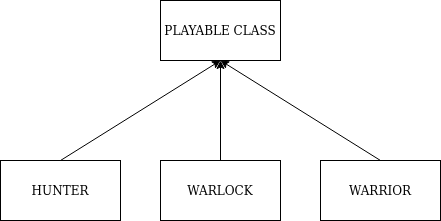
\includegraphics[scale=0.5]{imagens/heranca.png}
\caption{Herança Simples.} 
\label{fig:heranca}
\end{figure}

Uma hierarquia de classes utilizando Herança Simples é organizada como uma árvore, na qual cada nodo pode ter apenas um parente, ou seja, pode herdar de apenas uma classe. No caso, se uma entidade precisar herdar mais de um componente, este formato de árvore não é suficiente, sendo necessário o uso de Herança Múltipla. Neste tipo de herança, uma classe derivada pode extender de mais de uma classe pai.

Embora pareça uma solução fácil e simples no início, questões relacionadas ao uso de heranças múltiplas irão surgir. Um dessas questões é o problema do diamante, também conhecido como Deadly Diamond. Este é um problema de ambiguidade que ocorre quando duas ou mais classes, por exemplo, B e C herdam de uma classe A, e uma outra classe D herda de B e C, conforme a ilustração \ref{fig:deadlyDiamond}. Se existe um método em A no qual ambos B e C subscrevem e o método D não subscreve, então D vai herdar este método de B ou C?

\begin{figure}
\centering
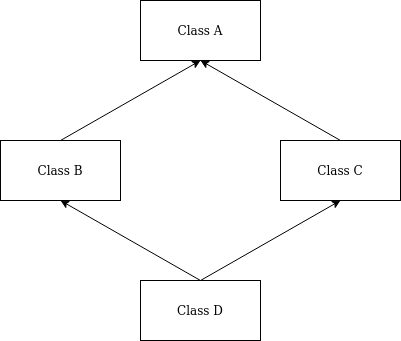
\includegraphics[scale=0.5]{imagens/deadly_diamond.png}
\caption{Deadly Diamond Problem.} 
\label{fig:deadlyDiamond}
\end{figure}

De acordo com Toni Härkönen, este tipo de Herança pode rapidamente se tornar trabalhosa para manter e expandir, uma vez que questões relacionadas a qual cópia da classe base será usada precisam ser resolvidas \cite{advantagesEcs}. Para resolver este problema, será necessário reorganizar a hierarquia de classes para se livrar do Deadly Diamond, provavelmente aumentando a repetição de código ou usando uma solução específica da linguagem de programação utilizada \cite{advantagesEcs}.

Outro problema no uso de Heranças é o acoplamento rígido da estrutura hierárquica de classes. Utilizando herança, um código com uma grande quantidade de entidades que herdam de outras entidades rapidamente vai possuir uma hierarquia de classes profunda. Alterar uma classe base, neste caso, pode causar efeitos colaterais indesejados em suas classes derivadas ou mesmo em todo o código \cite{composition}.

O problema citado anteriormente também é conhecido como \textit{Fragile base class}. Este é um problema de arquitetura da Programação Orientada a Objetos. Nele, as classes base são consideradas frágeis porque modificações aparentemente seguras na classe base, quando herdadas pelas classes derivadas podem causar um mal-funcionamento. Não dá para determinar se uma mudança é segura apenas examinando os métodos da classe base.

% falar sobre manutenibilidade

De acordo com Vittorio Romeo \cite{multiEcs}, considerando uma aplicação complexa ou um jogo que faz uso de uma arquitetura tradicionalmente orientada a objetos, as classes base são definidas como raízes de grandes hierarquias, das quais as entidades derivam. Com a adição de novos tipos de entidade, a complexidade do código aumenta, enquanto a capacidade de reutilização, flexibilidade e desempenho diminuem \cite{multiEcs}. 

Uma solução possível, segundo Toni Härkönen \cite{advantagesEcs}, é utilizar componentes ao invés de utilizar herança para agregar funcionalidades a um objeto. Resolvendo o problema do diamante e o problema do acoplamento rígido entre as classes.

Para Vittorio Romeo, uma abordagem alternativa mais poderosa consiste em usar um Design Orientado a Dados ou Composição, onde o código é projetado em torno dos dados e seu fluxo, e as entidades são definidas como um agregado de componentes \cite{multiEcs}.

O uso de Composição surge como uma alternativa ao uso de Herança.

\subsection{Composição}
A Composição permite a criação de tipos complexos combinando componentes de vários tipos, em vez de herdar de uma classe base ou pai \cite{composition}. Segundo Brian \cite{composition}, a composição contém instâncias de outras classes que implementam a funcionalidade desejada.

Fazendo uma analogia, é possível imaginar a Composição como um objeto montado de blocos de Lego. Várias peças de Lego (componentes) combinadas criam algo mais complexo, conforme mostra a figura \ref{fig:lego}. 

% como faço para citar uma imagem
\begin{figure}
\centering
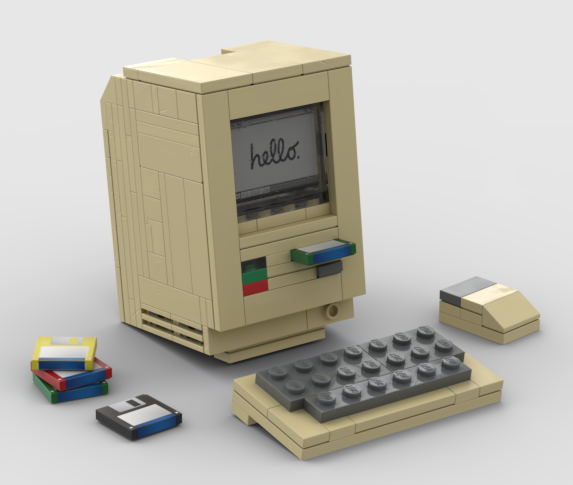
\includegraphics[scale=0.5]{imagens/macintosh.png}
\caption{Objeto construído combinando vários componentes.} 
\label{fig:lego}
\end{figure}

Este tipo de solução considera as mudanças futuras que podem ocorrer nos requisitos do software. Utilizando composição, não é necessário fazer uma reestruturação da árvore de classes, é possível simplesmente adicionar um novo componente à classe composta, sem modificar a superclasse para adaptar as mudanças \cite{composition}.

A figura \ref{fig:component} mostra como ficaria essa solução que utiliza um padrão conhecido como Object-Oriented Composition. Neste padrão, as entidades são compostas de pequenos componentes, que acrescentam funcionalidades a entidade. Estes componentes podem ser reutilizados em várias outras entidades. 

Um problema desta abordagem é que ela não dá suporte a separação dos dados e da lógica, ou seja, o componente possui os dados e a lógica na mesma estrutura. Uma outra abordagem proposta é utilizar um design que gerencia os dados de maneira mais eficaz, utilizando o padrão Entity Component System.

\begin{figure}
\centering
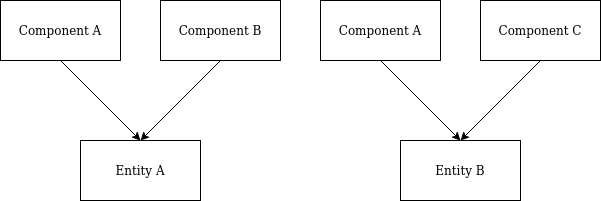
\includegraphics[scale=0.5]{imagens/component.png}
\caption{Object Oriented Composition.} 
\label{fig:component}
\end{figure}




\section{Entity-Component-System}
\label{sec:ECS}

O desenvolvimento de aplicações de tempo real e de jogos pedem por um sistema de gerenciamento de entidades que seja flexível e eficiente. \textit{Entity-Component-System} (ECS) é um padrão de desenho (\textit{design pattern}) de software amplamente utilizada em jogos, tipicamente em sistemas interativos em tempo-real (e.g. jogos do tipo MMO, \textit{Massive Multiplayer Online}) \cite{wiebusch2015decoupling}. 


Nesse padrão, objetos da simulação são transformados em \textit{entidades}. Uma entidade está relacionada a um conceito específico (e.g. uma parede, um robô, uma pessoa etc), com dados relacionados. Entidades podem ser criadas e destruídas ao longo da execução da simulação, e são usados apenas como identificadores. Cada entidade identifica uma coleção de \textit{componentes}. 

Um componente, por sua vez, armazena dados, mas tipicamente não implementa nenhuma lógica \cite{advantagesEcs}. Componentes também podem ser adicionados ou removidos durante a execução da simulação, alterando o estado da entidade à qual pertencem. Componentes representam algum atributo, estado ou capacidade da entidade (e.g. Posição, Velocidade, Sensores, etc). Dessa forma, o padrão ECS consegue separar dados da lógica da aplicação.

A lógica da simulação está nos \textit{sistemas}, que modificam os dados de componentes de acordo com seu objetivo \cite{multiEcs}. Em outras palavras, em vez de focar diretamente em uma entidade, os sistemas estão interessados em grupos de componentes que possuem os mesmos aspectos do sistema e que serão processados para realizar uma determinada tarefa \cite{advantagesEcs}. Cada sistema age de maneira independente de outros sistemas sobre um conjunto de componentes que lhe interessa. Ao mudar valores dos componentes, os sistemas efetivamente mudam o estado da simulação. O estado da simulação é o conjunto de estados de todos os componentes de todas as entidades presentes na simualção. Ele é alterado apenas pelos sistemas, cada um alterando uma pequena parte desse estado global. 

A figura \ref{fig:ecs} mostra o funcionamento de um sistema que usa o \textit{ECS}. Neste exemplo existem duas entidades: Robot e RechargeStation. A entidade Robot possui um componente Battery, Collidable, Velocity e Position e a entidade RechargeStation possui os componentes Station, Collidable e Position. As entidades serão discutidas na seção Entity e os componentes serão abordados na seção Components. 

\begin{figure}
    \centering
    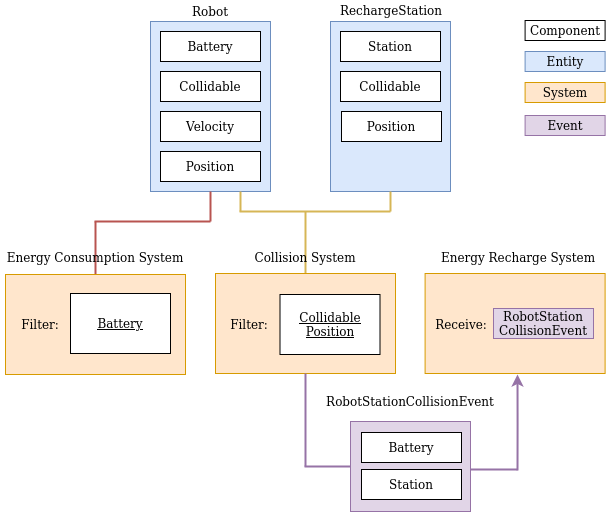
\includegraphics[width=\textwidth]{imagens/ecs.png}
    \caption{Exemplo de sistema construído no padrão ECS.} 
    \label{fig:ecs}
\end{figure}

O exemplo \ref{fig:ecs} apresenta dois sistemas. \texttt{Energy Consumption System} é responsável por consumir (decrementar) o total de energia de todas as entidades que possuem o componente \texttt{Battery}, sendo que nesse caso apenas a entidade Robot possui este componente. \texttt{Collision System} é responsável por verificar e notificar colisões entre entidades da simulação. Se ocorrer uma colisão entre uma entidade \texttt{Robot} e uma \texttt{RechargeStation}, significa que esse \texttt{Robot} quer recarregar a sua bateria. Sistemas são uma parte importante do simulador e são discutidos em maior detalhe na Seção \ref{sec:systems}.

% GIO: Achei muito detalhe isso aqui. Não creio que precisa ser incluído, mas não quis apagar. Talvez não concordem em remover
% e, portanto, o Collision System enviará uma notificação chamada RobotStationCollisionEvent para o sistema Energy Recharge System. O Energy Recharge System vai receber a notificação enviada e será responsável por recarregar a energia desse robô que está colidindo com a estação de recarga, incrementando o total de sua bateria. A parte de eventos, que é responsável por enviar notificações entre sistemas será melhor discutida na seção Eventos.

Essa organização permite grande modularização e separação de lógica entre as diferentes partes do sistema. Cada sistema (ou conjunto de sistemas) e seu conjunto de componentes associados pode ser adicionado ou removido do simulador conforme necessário, de maneira independente. Por exemplo, um sistema comunicação entre diferentes robôs pode ser implementado como um componente que guarde uma fila de mensagens e pode ser adicionado à cada robô, associado à dois sistemas: um sistema que faça a entrega das mensagens de um robô para o outro, e outro sistema que processa as mensagens de cada robô. Note que se o processamento não for adequado à uma simulação, basta trocar aquele sistema por outro que seja adequado. Além disso, se alguma simulação não faz uso desse sistema de mensagens, basta removê-lo do simulador completamente, deixando a simulação mais leve.

Uma outra vantagem de utilizar o padrão ECS é a flexibilidade de adicionar ou remover capacidades das entidades durante a execução da simulação. Como cada entidade é simplesmente uma coleção de componentes, é possível associar certas capacidades dos robôs (e.g. sensores, atuadores) à presença ou ausência de certos componentes naquela entidade. Por exemplo, dada a existência de um componente \texttt{camera} e um sistema associado que simule a captura de imagens, qualquer entidade que possue esse componente vai possuir a capacidade de coletar imagens via componente camera. Além disso, al simular falhas catastróficas em componentes, basta remover o componente da entidade sendo analisada.

Apesar dessas vantagens, como apontado por Wiebush \cite{wiebusch2015decoupling}, o uso de ECS pode trazer complicações de compatibilidade entre sistemas desenvolvidos de maneira indepentente, como uso de componentes incompatíveis, e dificuldade em conhecer qual sistema é responsável por determinada funcionalidade e como utilizá-la. detalhes de como esses problemas foram sentidos durante o desenvolvimento do projeto e medidas tomadas para mitigá-los são discutidas no capítulo \ref{chapter:hmr_sim}.

Foi utilizada a biblioteca \texttt{esper} para suporte do padrão ECS. Esper é uma biblioteca de ECS leve com foco em performance, escrita na linguagem Python por Benjamin Moran \cite{esper}. Ela cria uma classe \texttt{World} que mantém uma lista de entidades e de todos os componentes para cada entidade. Um componente pode ser qualquer estrutura em Python, no caso do projeto foram usadas classes (i.e. \texttt{class}). É possível ainda adicionar sistemas à classe \texttt{World}, que são implementados como funções, convencionalmente chamadas \texttt{process}. Alguns dos sistemas do projeto são adicionados ao \texttt{World}. \texttt{esper} também fornece funções que facilitam a obtenção de componentes ou conjuntos de componentes das entidades salvas, criação e remoção de entidades e componentes, e gerencia a execução dos sistemas.


\section{Técnicas de Simulação}
\label{sec:simulation_techniques}

Uma técnica de simulação bem estabelecida é a de tempo discreto com intervalo de incremento fixo \cite{belanger2010aboutsimulation}. Nesse modelo, o estado de um sistema no tempo $t_{i+1}$ é uma função do estado do sistema no tempo $t_i$. Cada variável que compõe o estado do sistema é uma função de variáveis e estados até o momento anterior. O incremento de tempo da simulação entre $t_i$ e $t_{i+1}$ é sempre o mesmo, e pré-definido.

Se o tempo $t_{calc}$ necessário para computar o estado $t_{i+1}$ do sistema a partir do estado $t_i$ é menor do que o tempo do incremento $t_{incr}$, então a simulação será computada mais rápido do que o tempo do relógio (e.g. o tempo real); da mesma forma, se $t_{calc} > t_{incr}$, então a simulação é computada mais devagar do que o tempo do relógio. Essas situações são conhecidas como simulação \textit{offline} \cite{belanger2010aboutsimulation}, porque não há sincronia entre o tempo da simulação e o tempo do relógio. Essa é uma situação aceitável para este projeto, onde o objetivo é obter a simulação desejada no menor tempo possível.

Essa técnica de simulação é indicada para simular sistemas que mudam constantemente, como por exemplo a temperatura de um ambiente ao longo do tempo, ou um sinal recebido por um sensor que trabalha a uma frequência conhecida. No entanto o  "relógio" da simulação é sincronizado, e todas as funções do estado são processadas a cada incremento de tempo, o que pode levar a cálculos desnecessários. Por exemplo, em uma simulação que involva uma função que altera temperatura de uma sala a cada 200ms, e um sensor que registra a temperatura da mesma sala com leituras a cada 100ms, a função que altera temperatura deve ser executada em todos os incrementos de tempo, que devem ser no máximo 100ms para suportar a leitura do sensor. Nesse cenário, metade das chamadas à função de alterar temperatura não afeta o estado do sistema, mas ainda tem que ser processadas.

Outra técnica de simulação é por eventos discretos (DES, \textit{Discrete Event Simulation}) \cite{matloff2008desintro}. Nesse modelo uma fila de eventos é processado um por vez, e cada estado $s_{i+1}$ é o resultado de processar o evento no topo da fila sobre o estado $s_i$. Um evento $e$ possui um tempo $t$ e uma função $f$ que altera o estado, e potencialmente cria outros eventos, que serão adicionados à fila. A fila de eventos é uma fila de prioridades ordenada pelo tempo $t$ de cada evento, sendo que o tempo de cada novo evento gerado pode ser igual ou maior que o tempo do evento que o gerou (nunca menor, porque não se pode alterar o passado da simulação). O tempo da simulação corresponde ao tempo $t$ do evento atual sendo processado, e como os eventos são ordenados pelo tempo, ele só será incrementado quando todos os eventos naquele tempo foram processados.

Diferentemente da simulação com intervalo de incremento fixo, onde as mesmas funções são executadas em intervalos conhecidos de tempo, na simulação do tipo DES funções diferentes alteram o estado da simulação, e o tempo da simulação no estado $s_i+1$ não depende apenas do estado $s$, mas também do evento sendo processado. Esse novo tempo pode não crescer de maneira uniforme ao longo da simulação. Essa técnica é adequada para simular sistemas que mudem de maneira infrequênte ao longo do tempo, por exemplo o inventário de um armazém \cite{belanger2010aboutsimulation}, ou a operação de robôs de serviço dentro do armazém. 

A simulação de incremento fixo de tempo pode ser implementada utilizando a técnica de eventos discretos, desde que os eventos sejam criados com tempos que possuam um intervalo constante. Uma outra característica interessante que pode ser alcançada com eventos discretos é separar a função em subsistemas que são executados de maneira independente e assíncrona. Retomando o exemplo da sala que muda de temperatura e possui o sensor, cada evento de leitura do sensor pode criar o próximo evento de leitura para o tempo $t + 100ms$; de forma similar cada evento de mudança de temperatura cria um novo evento de mudança para o tempo $t + 200ms$. Dessa forma, evita-se o problema de funções de alteração do estado da simulação tendo que ser executadas antes da hora.

O simulador utiliza a técnica de simulação de eventos discretos, através da biblioteca \texttt{simpy} \cite{simpy}. Esse framework de simulação DES é baseado em processos e faz todo o gerenciamento dos eventos e sua execução. A simulação acontece dentro de um ambiente, onde diversos processos interagem entre si e com o ambiente através de eventos. QUalquer função geradora em Python pode ser um process no simpy.

Esse framework também tem suporte para recursos (\textit{Resources}), que são compartilhados entre os processos. Recursos podem simular desde recursos a serem disputados (i.e. uma impressora, uma estação de carga) até recursos que são armazenados em contâiners (i.e. 10L de aguá de um reservatório com capacidade para 10000L). Recursos podem ainda ser preemptivos, ou filtrados de algum contâiner. Essa última capacidade foi bastante utilizada para a comunicação entre sistemas do simulador, como será discutido no Capítulo \ref{3_HMR_sim}.




%\subsection{Data-Oriented Design}
%No desenvolvimento de softwares computacionalmente mais pesados, um %problema frequente é o desempenho, que faz com que o tempo de execução %do programa para diferentes tarefas parem por tempos inaceitáveis %\cite{advantagesEcs}. Podem existir diferentes motivos para isso %ocorrer, como, por exemplo, algoritmos não otimizados, mas este não é o %principal caso. Para Toni Härkönen, é bastante comum que a lentidão %seja causada pelo gerenciamento ineficiente da memória. Uma solução %para este problema é utilizar um design que gerencia os dados de %maneira eficaz, portanto, o autor sugere uma mudança de pensamento %orientado a objetos para o design orientado a dados %\cite{advantagesEcs}.

% Falar sobre manutenibilidade e extensibilidade.

\subsection{Comunicação entre sistemas}
Um sistema muitas vezes terá a necessidade de se comunicar com outros sistemas. O uso de eventos dá suporte para estas comunicações.
\subsubsection{Eventos}
Uma parte importante das arquiteturas de softwares voltadas a jogos são os Eventos.
Eventos são ações que podem ser geradas quando um determinado comportamento ocorre em um determinado sistema, sendo enviados para um ou mais sistemas que terão como uma de suas atividades tratar a ocorrência dessas ações. Por exemplo, um evento de colisão, no qual duas entidades podem se colidir e quando isso ocorrer será enviado um evento para um Sistema responsável por tratar essa ocorrência.

Existem diferentes formas de tratar a ocorrência de eventos e muitas bibliotecas que lidam com \textit{Entity Component System} possuem um sistema de gerenciamento capaz de tratá-los. Também existem diferentes bibliotecas em várias linguagens para o tratamento de eventos (não apenas para jogos). Em python, por exemplo, existe a biblioteca PyDispatcher, que fornece um serviço centralizado para entrega de mensagens a objetos registrados \cite{pydispatcher} e também tem a biblioteca \textit{zope.event} \cite{Zope} que segue o padrão \textit{Observer}, entre várias outras bibliotecas.

Utilizando o padrão Observer é possível enviar a notificação da ocorrência de um evento para sistemas que ficam esperando a ocorrência desses eventos.

%Dependendo da forma como o tratamento de eventos ocorre, um determinado %sistema fica verificando a cada update todos os componentes %relacionados a ele para encontrar apenas as entidades necessárias para %realizar alguma lógica. Por exemplo: um sistema de Colisão vai procurar %todas as entidades que possuem um componente \textit{Collidable} e para %cada componente desse vai ter outra iteração por todos os componentes %\textit{Collidable} para verificar se ocorreu alguma colisão entre dois %componentes. 

%Dessa maneira o custo total de iterações para cada sistema acaba se %tornando maior conforme o número de sistemas e de entidades aumentam.

%Uma outra forma de lidar com eventos é utilizar padrões parecidos com o %\textit{Observer}, no qual não é necessário iterar toda vez sob todos %os objetos. Utilizando o padrão Observer é possível enviar a %notificação da ocorrência de um evento para sistemas que ficam %esperando a ocorrência desses eventos. 

\subsubsection{Observer Pattern}

\gio{Isso aqui é usado nos testes? Não vi muito sentido em explicar isso (do ponto de vista do simulador)}
O Padrão Observer é um Behavioral Pattern que define uma dependência entre objetos do tipo one-to-many de forma que quando um objeto muda o seu estado, todos os seus dependentes são notificados e atualizados de forma automática \cite{gamma1994design}.

O padrão \textit{Observer} permite definir um sistema de notificações no qual um objeto, conhecido como \textit{Subject}, pode enviar eventos para outros objetos, conhecidos como \textit{Observers}, que ficam esperando (observando) por essas notificações. Para isso, o \textit{Subject} mantém uma lista de dependentes do tipo \textit{Observers} e quando ocorre uma mudança no seu estado é enviado uma notificação para todos os \textit{Observers} dessa lista.

Este tipo de interação também é conhecida como Publish-Subscribe \cite{gamma1994design}. O Subject é o Publisher (publicador) das notificações e os Observers podem ser descritos como Subscribers.

Para diminuir o acoplamento e para que o \textit{Publisher} não precise saber da implementação de todos os \textit{Subscribers} é importante que se utilize uma mesma interface entre os \textit{Subscribers} e que o \textit{Publisher} possa se comunicar com eles através dessa interface \cite{observer}.

A estrutura do Observer Pattern é ilustrada pela figura \ref{fig:observer}. Este exemplo possui os seguintes participantes:
\begin{itemize}
    \item Subject:
        \begin{itemize}
            \item Guarda os estados de interesse dos Observers;
            \item Provê um meio de registrar e de cancelar o registro de um observer;
            \item Envia notificações para os observadores quando ocorre mudanças no estado;
            \item Guarda uma lista de Observers.
        \end{itemize}
    \item Observer:
        \begin{itemize}
            \item Define a interface para atualizar os objetos que serão notificados da mudança no Subject.
        \end{itemize}
    \item ConcreteObserver:
        \begin{itemize}
            \item Implementa a interface de update (atualização) do Observer.
        \end{itemize}
\end{itemize}

\begin{figure}
\centering
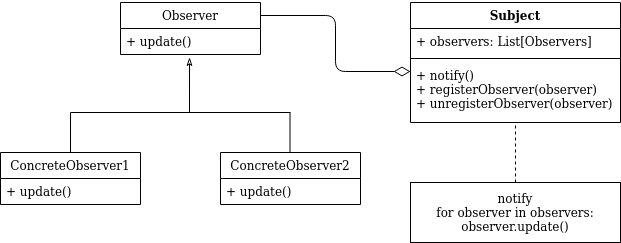
\includegraphics[width=\textwidth]{imagens/observer.png}
\caption{Observer Pattern.} 
\label{fig:observer}
\end{figure}

%TODO não se referencia Wikipédia em trabalho academico. A referência padrão em design patterns é o livro "Design Patterns: Elements of Reusable Object-Oriented Software - Erich Gamma, Richard Helm, Ralph Johnson, and John Vlissides, with a foreword by Grady Booch."

%Atualmente o projeto utiliza duas formas de tratamento de eventos: o %tratamento de eventos do gerenciador de ECSs Esper e o tratamento de %eventos do Simpy.

%O tratamento de eventos do Esper segue um padrão de comunicação entre %componentes. O sistema responsável por tratar um determinado tipo de %evento faz uma busca por todas as entidades que possuem certos tipos de %componentes. Por exemplo, um Sistema de Colisão precisa acessar todas %as entidades que possuem todos os três componentes: Collidable, %Position e Velocity.

% section simulacao
% subsection simulacao utilizando ECS

\section{Behavior Driven Development}
O BDD é um conjunto de práticas da Engenharia de Software que tem como propósito melhorar a qualidade do código e a entrega de um software correto \cite{bddInAction}. O BDD baseia-se em práticas Ágeis e do Lean, utilizando principalmente técnicas do DDD (Domain-Driven Design) e do TDD (Test-Driven Development).

O BDD propõe o uso de uma linguagem que é entendível por todos os stakeholders. Desta forma, todos os envolvidos vão utilizar essa linguagem para descrever as funcionalidades do software, que serão descritas em vários arquivos que terminam com o sufixo .feature. Uma das ideias do BDD é utilizar estes arquivos como uma forma de documentação e também para testar os vários comportamentos do software.

As features e os cenários dela descrevem os requisitos do software e serão usadas como casos de teste. Cada arquivo .feature será responsável por descrever um ou mais cenários.

Os cenários são compostos de várias regras e cada regra pode ser mapeada a um método que vai verificar se ela é executada corretamente. Para a criação dos cenários é utilizada linguagens que podem ser entendidas por todos os stakeholders, um exemplo é a linguagem Gherkin.

Uma feature pode ser especificada da seguinte forma \cite{BDDthesis}:

\textbf{Feature}: breve descrição da funcionalidade

\textbf{Background}: agrupa regras que são comuns em todos os cenários.

\textbf{Scenario}: descrição de um cenário específico da funcionalidade.

\hspace{1cm}\textbf{Given} uma pre-condição

\hspace{1cm}\textbf{And} outra pre-condição

\hspace{1cm}\textbf{When} ocorre uma ação

\hspace{1cm}\textbf{And} outra ação ocorre

\hspace{1cm}\textbf{Then} é obtido um resultado testável

Cada keyword do Gherkin\footnote{https://cucumber.io/docs/gherkin/reference/} descrita acima é responsável por:
\begin{itemize}
    \item \textbf{Feature}:
    O propósito da keyword feature é dar uma descrição de alto nível de uma funcionalidade do sistema e agrupar os cenários relacionados a esta feature.
    \item \textbf{Background}:
    Quando uma ou mais regras Given estão sendo repetidas em todos os cenários, elas podem ser agrupadas na seção do Background. As regras agrupadas nesta seção serão executadas antes dos cenários.
    \item \textbf{Scenario}:
    A keyword Scenario descreve uma regra de negócio da funcionalidade e é composto por várias regras Given/When/Then.
    \item \textbf{Scenario Outline}:
    Permite executar um cenário várias vezes e a cada vez utiliza exemplos de valores diferentes. Os valores serão definidos com a keyword Examples.
    \item \textbf{Examples}:
    Permite criar uma tabela de exemplos. Cada coluna da tabela representa uma variável e cada linha vai conter um valor diferente para a variável. Estes exemplos podem ser usados quando um cenário é executado várias vezes, dessa forma, a cada vez que um cenário é executado é lida uma linha da tabela de exemplos.
    \item \textbf{Steps}
    Descreve os passos necessários para completar um cenário. Estes passos podem ser dos seguintes tipos:
    \begin{itemize}
        \item \textbf{Given}:
        Define um estado inicial antes de começar a testar. Nesta etapa podem ser feitas instâncias de objetos, configurações de banco de dados, busca por uma página da web, entre outras configurações necessárias para deixar o sistema em um estado inicial.
        \item \textbf{When}:
        Define um evento ou uma ação que será realizada no sistema que está sendo testado. Esta ação pode ser feita por uma pessoa ou por um outro sistema. 
        \item \textbf{Then}:
        Descreve o resultado esperado da execução das etapas anteriores. Nesta etapa será realizado o assert para verificar se o output recebido é igual ao output que era esperado.
        \item \textbf{And/But}:
        Serve como um sinônimo para o passo anterior a ele e é utilizado para evitar várias escritas do Given/When/Then.
    \end{itemize}
    
    
\end{itemize}

\gab{TODO ao invés de image, usar listing com highlight para Gherkin
% ref: https://gist.github.com/nsommer/9a04f6ebc6ea8b9f5b816becb97e7d9b
}

\begin{figure}
\centering
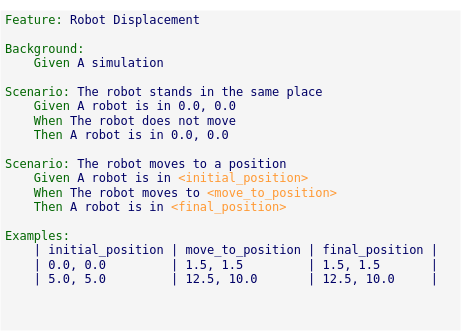
\includegraphics[width=\textwidth]{imagens/bddExample.png}
\caption{Exemplo de um arquivo .feature} 
\label{fig:bddExample}
\end{figure}

A figura \ref{fig:bddExample} mostra um exemplo de um arquivo .feature.

Um problema que o BDD tenta resolver é a comunicação entre os times e demais stakeholders e a perda de informações das features ao longo dos diversos processos. Por exemplo, utilizando o BDD, quando uma pessoa da área de negócios pede por uma nova feature, ela vai se reunir com o time de desenvolvedores e de testadores e vai explicar os requisitos dessa nova feature. Nesta reunião, todos os envolvidos vão traduzir essas especificações, utilizando a linguagem Gherkin, em cenários e regras que podem ser entendidos por todos os envolvidos. Os diversos cenários e regras descritos vão guiar o desenvolvimento da feature e vão servir como casos de teste \cite{bddInAction}.

De acordo com \cite{bddInAction}, o BDD vai ajudar o time a focar na identificação, no entendimento e na implementação das features que realmente importam para os clientes.


\section{Simulações Robóticas}

\gio{ Acho essa seção desnecessária. Tudo que tem aqui já foi falado na introdução. Melhor falar tudo lá, até porque faz parte do contexto do projeto.}

Simulações robóticas são ferramentas importantes para o processo de design, de prototipação, de desenvolvimento e da verificação e validação de um sistema robótico. Sendo uma opção mais viável e barata do que fazer testes em campo \cite{robotSimulation}. Essas simulações são usadas na maioria das vezes para fazer testes, podendo ser usadas para testar algoritmos, componentes, sistemas multi-robôs, dentre outros tipos de sistemas. O artigo \cite{robotSimulation} mostra que os desenvolvedores enxergam valor em utilizar simulações para testes e que esses desenvolvedores utilizam simulações quando é impraticável fazer os testes em um hardware ou outro ambiente real.


\subsection{Dificuldades}
Mesmo tendo um bom potencial, o uso de simulações possui vários desafios e dificuldades, conforme foi relatado por desenvolvedores da área da robótica \cite{robotSimulation}.

As principais dificuldades relatadas \cite{robotSimulation} ao usar simulações foram:

\begin{itemize}
    \item \textbf{Diferença entre realidade e simulação}: Existe uma grande discrepância entre a realidade e a simulação. Muitas vezes existe uma inadequação da representação da física no simulador ou a produção de comportamentos não realistas.
    \item \textbf{Complexidade}: É referente às dificuldades adicionais na usabilidade do simulador. Serão gastos tempo e recursos que poderiam ser gastos em outras atividades. Conforme relatado, sairia mais fácil e mais acurado configurar e testar em um sistema físico real.
    \item \textbf{Falta de funcionalidades}: Os simuladores não possuem todas as funcionalidades desejadas pelo desenvolvedor ou se possuem são bastante caros. Cada simulador é bom em um determinado aspecto, mas nenhum é bom em todos eles. 
    \item \textbf{Documentação}: Falta de documentação ou documentação errada.
\end{itemize}

Dificuldades relacionadas a construção de testes \cite{robotSimulation}:
\begin{itemize}
    \item \textbf{Reprodutibilidade}: É difícil repetir o resultado de uma simulação, pois ela é não determinística.
    \item \textbf{Construção de cenários e ambientes}: Os desenvolvedores relataram ter dificuldade ao criar os cenários para os testes.
\end{itemize}

Desafios que afetam a automação dos testes \cite{robotSimulation}:
\begin{itemize}
    \item Não ser possível rodar os testes sem desabilitar a GUI é uma das maiores dificuldades da automação dos testes.
    \item Rodar a simulação sem intervenção manual.
    \item Não ter uma terminação clara da simulação.
    \item Interfaces instáveis.
\end{itemize}


% \chapter{Evaluation}
% \label{chap:evaluation}
% \input{parts/evaluation}
% %\input{end/evaluation}

% \chapter{Related Work}
% \label{chap:related}
% \input{parts/related}

% \chapter{Conclusion}
% \label{chap:conclusion}
% \input{parts/conclusion}
%\input{end/conclusion}

\postextual
\anexos


\bibliographystyle{plain}
\bibliography{bibliografia}
\end{document}
